


\documentclass[11pt]{article} 
\topmargin=0.0in 
\oddsidemargin=0.0in 
\evensidemargin=0in 
\textwidth=6.5in 
\marginparwidth=0.5in
\headheight=0pt 
\headsep=0pt 
\textheight=9.0in 
\usepackage{multicol}
\usepackage{graphicx}
\usepackage{vwcol}
\graphicspath{{./images/}}

\begin{document}
\centerline{\Large Manav Guglani} 
\noindent 
\line(1,0){470}
\\  
 \parbox[t]{5cm}
{305, BH-7,\\
	NIT Uttarakhand\\
	Srinagar \\
	Garhwal-246174\\
	Uttarakhand}


\hspace{7cm}
\parbox[t]{8cm}
{Contact: 9548899230\\
email:	manav.ece14@nituk.ac.in\\
	\vspace{1pt}
	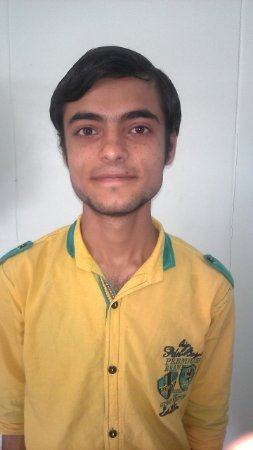
\includegraphics[scale=.2]{manav.jpg}
}
\section*{Objective}
\Large To excel in embedded systems and robotics and using this excellence to create useful products for growth of India. 
\section*{Education} 
\begin{tabular}{|c|c|c|c|c|}
	\hline
	Degree & College/School & University & Passing Year & cgpa or \% \\
	\hline
	B.tech & NIT Uttarakhand & NIT Uttarakhand & 2018 & 9.18\\
	\hline
	Intermediate & B.J.S. Public School & CBSE & 2013 & 90.40 \% \\
	\hline
	High School & B.J.S. Public School & CBSE & 2011 & 9.0 \\
	\hline
\end{tabular}
\section*{Projects}  
\begin{enumerate}
	\item Gas leakage detection robot
	\item Interfacing TSOP IR receiver with FPGA by Using Verilog HDL
	\item Wireless control of home appliances
	\item Self balancing robot
\end{enumerate}	
\section*{Training and Internship}  
\begin{itemize}
	\item	Application of embedded systems in robotics and automation at Roboshack Microtronics Pvt. Ltd. 
\end{itemize}
\section*{Research Publication}
\section*{Technical skills}   
\begin{itemize}
	\item C
	\item verilog HDL
	\item 8085 assembly
\end{itemize} 	
\section*{Soft skills}  
\begin{enumerate}
	\item Adaptability
	\item Problem solving
	\item Dedicated
	\item Perseverance
\end{enumerate}
\section*{Extra-curricular activities}  
\begin{itemize}
	\item College Technical meet (both 2015 and 2016)
	\item speech competition in college
	\item e-yantra robotics competition (both 2015 and 2016)
\end{itemize}
\section*{Co-curricular activities}  
\begin{enumerate}
	\item Doing pranayama and yogasana
	\item Teaching friends
\end{enumerate}

\end{document}
